\section{Gallium Arsenide --- MLWFs for the valence bands}
\label{sec1:GaAs}
\begin{itemize}
\item Outline: {\it Obtain and plot MLWFs for the four valence bands of GaAs.}
\end{itemize}

\begin{figure}[h!]
\centering
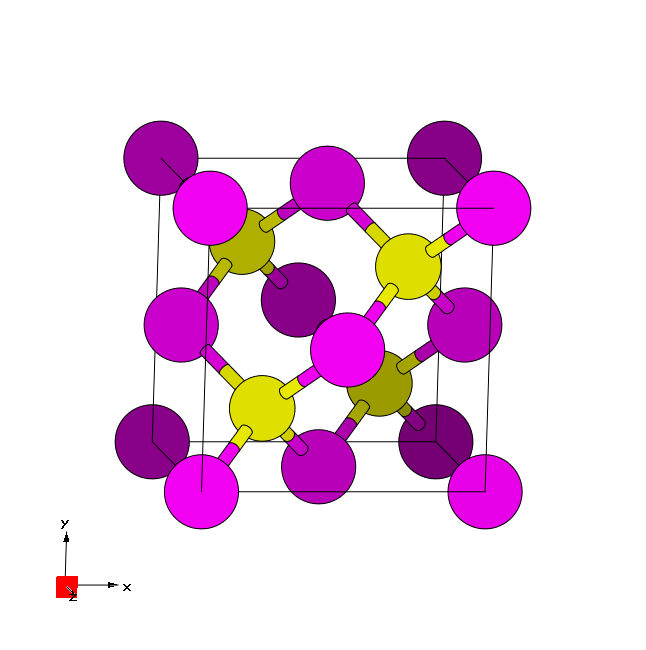
\includegraphics[width=0.25\columnwidth,trim={45pt 45pt 55pt 55pt},clip]{figure/example01/GaAs.png}
\caption{Unit cell of GaAs crystal plotted with the \xcrysden{} program.}
\label{fig1}
\end{figure}

\begin{enumerate}

\item {\it Inspect the output file {\tt gaas.wout}.}

\Tab{tab1.1} shows the converged values (after 20 iterations) for a $2\times2\times2$ \bfk-point mesh of the total spread functional $\Omega$ and its three components, \ie{} the gauge-invariant component $\Omega\tinysub{I}$, the off-diagonal component of the gauge-dependent part $\Omega\tinysub{OD}$, and the diagonal component of the gauge-dependent part $\Omega\tinysub{D}$, respectively. These can be found at the end of the {\tt gaas.wout} file, from the line starting with {\tt Final State}. You will find the \MLWF{} centres and their spreads together with the information on the spread functional components as reported below, and summarized in tab.\ref{tab1.1}.
\begin{tcolorbox}[sharp corners,boxrule=0.5pt]
{\small
\begin{verbatim}
 Final State
  WF centre and spread    1  ( -0.866253,  1.973841,  1.973841 )     1.11672024
  WF centre and spread    2  ( -0.866253,  0.866253,  0.866253 )     1.11672024
  WF centre and spread    3  ( -1.973841,  1.973841,  0.866253 )     1.11672024
  WF centre and spread    4  ( -1.973841,  0.866253,  1.973841 )     1.11672024
  Sum of centres and spreads ( -5.680188,  5.680188,  5.680188 )     4.46688098
  
         Spreads (Ang^2)       Omega I      =     3.956862958
        ================       Omega D      =     0.008030049
                               Omega OD     =     0.501987969
    Final Spread (Ang^2)       Omega Total  =     4.466880976
  -----------------------------------------------------------------------------
\end{verbatim}
}
\end{tcolorbox}
The geometric centre lies along the Ga-As bond, slightly closer to As than Ga. To see this, we introduce a measure $\beta$ defined as 
$$\beta \triangleq \frac{d\tinysub{Ga-MLWF}}{d\tinysub{Ga-As}},$$

where $d\tinysub{Ga-MLWF}$ is the distance of the Ga atom placed in the origin and the \MLWF{} centre (along the Ga-As bond), and $d\tinysub{Ga-As}$ is the Ga-As bond length, \cf{} Ref.~\cite{marzarivanderbilt1997}. A value of 0.5 corresponds to the \MLWF{} centre being equidistant from the Ga atom and As atom. 
In our case, we find: $$\beta = \frac{d\tinysub{Ga-MLWF(2)}}{d\tinysub{Ga-As}} = \frac{0.866253\sqrt{3}}{1.4200\sqrt{3}} \approx 0.61 .$$
Maximum RAM allocated for the wannierisation was 0.06Mb.

\begin{table}[ht!]
\centering
\captionsetup{width=.5\textwidth}
\caption{Converged values of the components of spread functional and their sum, given in \angsqd{}. Here $\beta$ is the distance of the Ga atom placed in the origin and the \MLWF{} centre (along the Ga-As bond) as a fraction of the Ga-As bond length $2.4595\si{\angstrom}$.}
\begin{tabular}{@{} llllll @{}}\toprule[1.5pt]
MP mesh & $\Omega$ & $\Omega\tinysub{I}$ & $\Omega\tinysub{OD}$ & $\Omega\tinysub{D}$ & $\beta$\\\midrule
$2\times2\times2$ & 4.467 & 3.957 & 0.502 & 0.008 & 0.610 \\\bottomrule[1pt]
\end{tabular}\label{tab1.1}
\end{table}

\item {\it Plot the MLWFs.} 

In \Fig{fig1.2} are shown the four valence \MLWFs{} as plotted by \xcrysden{}, where we used the following parameters in the {\tt Tools} $\mapsto$ {\tt Data Grid} section: 

\begin{tcolorbox}[colback=blue!10,hbox,title=Xcrysden: {\tt Tools} $\mapsto$ {\tt Data Grid}]
{\tt 
Degree of triCubic Spline = 3;
Isovolume = 0.95;
Render +/- isovalue = yes
}
\end{tcolorbox}

\begin{figure}[h!]
\centering
\subfloat[$1\tinysup{st}$ valence \MLWF{}]{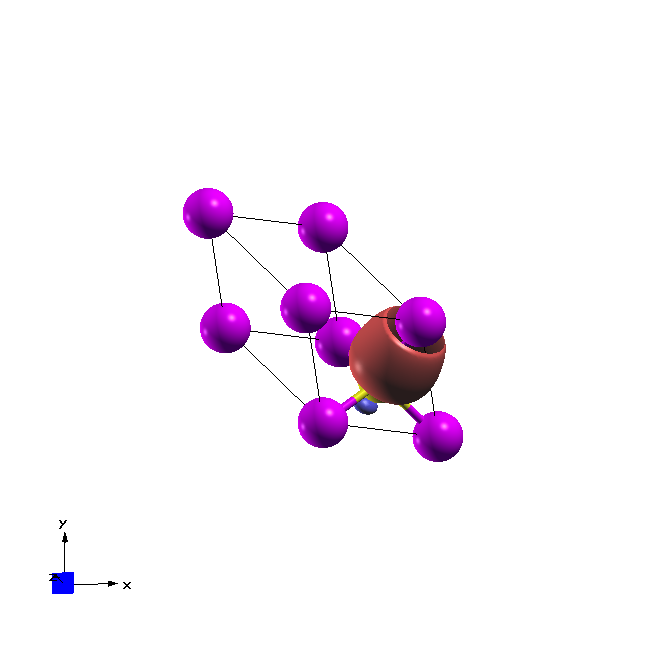
\includegraphics[width=0.25\columnwidth,trim={120px 120px 120px 120px},clip]{figure/example01/gaas_00001_rotate.png}}
\centering
\subfloat[$2\tinysup{nd}$ valence \MLWF{}]{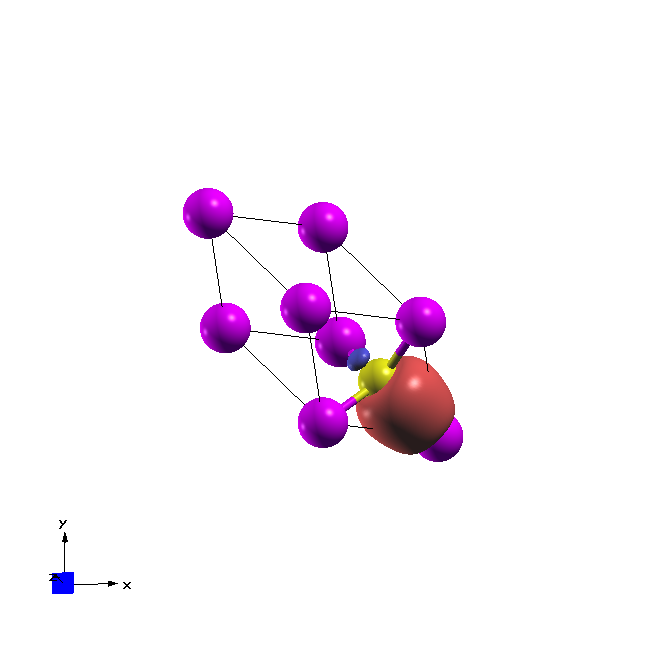
\includegraphics[width=0.25\columnwidth,trim={120px 120px 120px 120px},clip]{figure/example01/gaas_00002_rotate.png}}
\centering
\subfloat[$3\tinysup{rd}$ valence \MLWF{}]{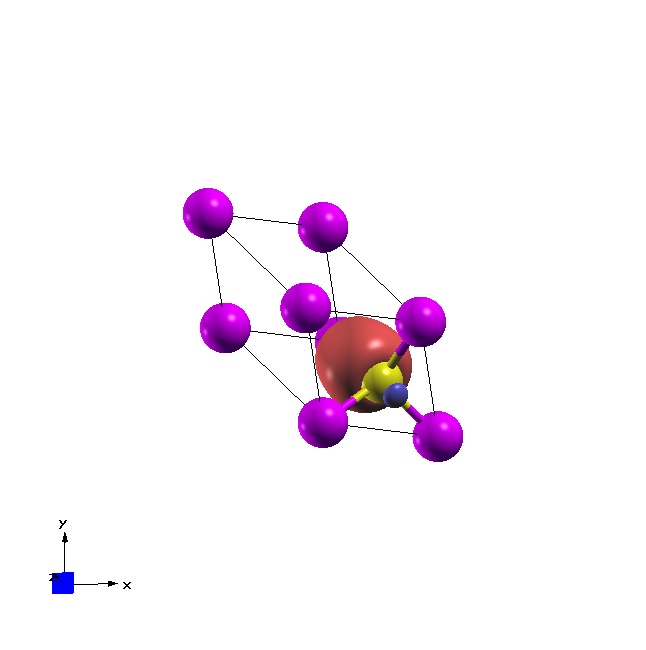
\includegraphics[width=0.25\columnwidth,trim={120px 120px 120px 120px},clip]{figure/example01/gaas_00003_rotate.png}}
\centering
\subfloat[$4\tinysup{th}$ valence \MLWF{}]{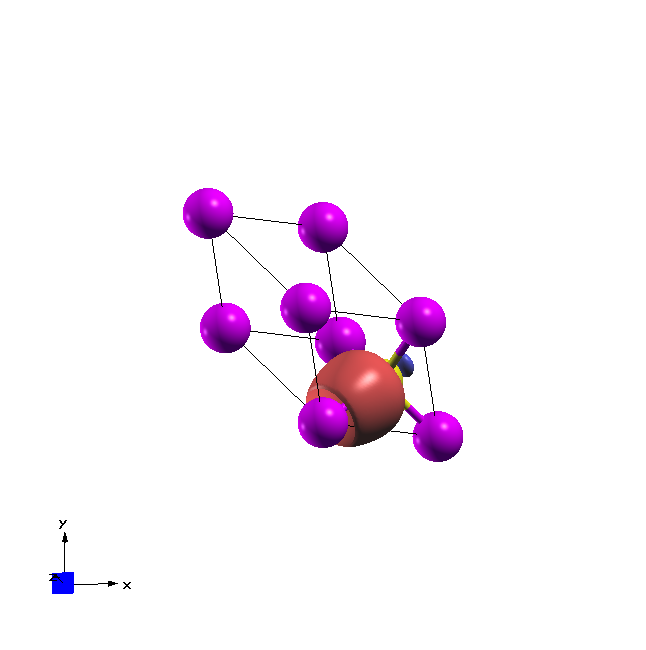
\includegraphics[width=0.25\columnwidth,trim={120px 120px 120px 120px},clip]{figure/example01/gaas_00004_rotate.png}}
\caption{Four valence \MLWFs{} for the Ga-As system plotted using the \xcrysden{} visualisation program.}\label{fig1.2}
\end{figure}

\item[Extra :] {\it Plot the 3$rd$ MLWFs in a supercell of size 3. Choose a low value for the isosurface (say 0.5). Can
you explain what you see?}

With \xcrysden{} we can also plot the $3\tinysup{rd}$ \MLWF{} to check its periodicity. The period in each direction is given by the spacing used to sample the first irreducible Brillouin zone, \ie{} the \bfk-point mesh. We used a $2\times2\times2$ \bfk-point mesh, hence we expect to find a periodic image of our \MLWF{} in a supercell which is 2 times larger than the unit cell along each direction. This is shown in \Fig{fig1.3}, where the $3\tinysup{rd}$ has been plotted using both the \xcrysden{} program and the \vesta{} program.   
\end{enumerate}

\begin{figure}[h!]
\centering
\subfloat[\xcrysden{}]{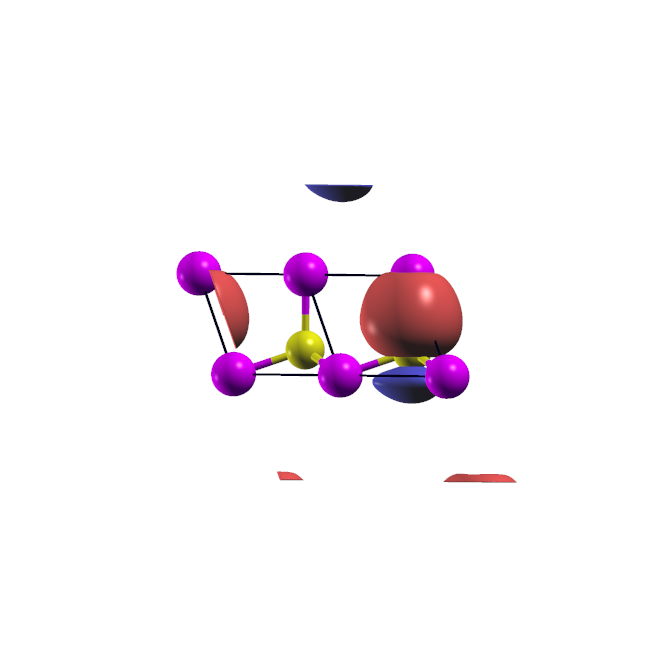
\includegraphics[width=0.5\columnwidth,trim={100pt 100pt 70pt 100pt},clip]{figure/example01/gaas_00003_cellsize3_xcrysden.png}}
\centering
\subfloat[\vesta{}]{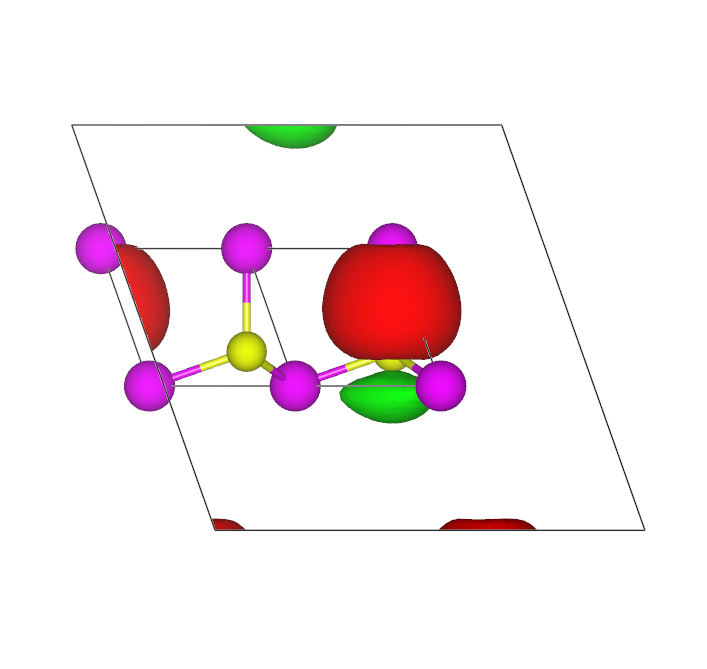
\includegraphics[width=0.5\columnwidth,trim={10pt 40px 30px 10px},clip]{figure/example01/gaas_00003_cellsize3_vesta.png}}
\caption{$3\tinysup{rd}$ \MLWF{} with a supercell value of 3 and for an isovalue of 0.5 using (a) \xcrysden{} and (b) \vesta.}\label{fig1.3}
\end{figure}
